\documentclass[11pt,a4paper,oneside]{article}

\usepackage{euler,amsthm,amsmath,amsfonts,graphicx,epigraph,indentfirst,enumerate,comment,listings,fontspec,color,subcaption,listings}
\usepackage{xeCJK}
\usepackage{hw}
\usepackage{pythonhighlight}
\usepackage{tikz}

\renewcommand{\hwtitle} {CS217 Homework 2}	
\renewcommand{\hwauthor}{Akina}
\renewcommand{\hwdate}{\today}

\begin{document}
\title{\hwtitle}
\author{\hwauthor}
\date{\hwdate}
\maketitle

\section*{Sorting Algorithms}
\begin{problem}{1}
	\statement
	Given an array $A$ of $n$ items (numbers), we can find the maximum with $n-1$ comparisons (this is simple).
	Show that this is optimal: that is, any algorithm that does $n-2$ or fewer comparisons will fail to find the maximum 
	on some inputs.
	\solution
	\begin{proof}
		Consider all the elements as vertices and comparisons as directed edges from larger to smaller ones, or the direction of the edge is arbitrary in the case of two elements are identical. Then consider how we conclude the maximum element: there's a path from the maximum element to every other element -- it's continuous inequations that mathematically proved the maximality.
		The simple algorithm forms a tree finally. Everytime it compares the current root and next element, adds an edge between them. Then the new root is decided according to the direction of the new edge.

		If there are $n - 2$ or fewer edges in the graph, the graph can not be connected since an edge can only decrease the number of connected components by 1. Howerver, in the beginning, we have $n$ components. What led to is that there are at least two components finally, which we don't really know their relations at all -- we can not conclude such inequation between any two vertices in different components, as well as the maximum element.
	\end{proof}
\end{problem}

\begin{problem}{2}
	\statement
	Let $A$ be an array of size $n$, where $n$ is even. 
	Describe how to find both the minimum and the maximum
	with at most $\frac{3}{2} n  - 2$ comparisons.
	Make sure your solution is {\em simple}, in describe it 
	in a clear and succinct way!

	\solution
	Life is short, I choose python.
\begin{python}
def min_max(a, n):
    small = []
    large = []
    for i in range(0, n, 2):
        res = a[i] > a[i + 1]
        small.append(a[i + res])
        large.append(a[i + 1 - res])
    return (min(small), max(large))
\end{python}
	First part, we make pair of every two ajancent number(their indexes are \(2n\) and \(2n + 1\) separately) and divides them by the result of comparisons which take $\frac n 2$ times.
	Second part we decide the maximum and minimum seperately, and both takes $\frac n 2 - 1$ comparisons(with use of the simple algorithm in Problem 1). In total, $\frac {3} {2} n - 2$ comparisons achieved.
\end{problem}
\begin{problem}{3}
	\statement
	Given an array $A$ of size $n = 2^k$, find the second largest element element
	with at most $n + \log_2(n)$ comparisons. 
	Again, your solution should be {\em simple}, and you should explain
	it in a clear and succinct way!
	
	\solution
	Life is even shorter, I choose python again.
\begin{python}
def second_max(a, n):
    b = [0] * (n + 1) + a
    for i in range(n - 1, 0, -1):
        b[i] = max(b[i * 2], b[i * 2 + 1])
    c = []
    x = 1
    while x < n:
        x *= 2
        x ^= b[x] != b[x >> 1]
        c.append(b[x ^ 1])
    return max(c)
\end{python}
	First part we do $n - 1$ comparisons to get the maximum element by a heap-like order, using an array of $2n$ elements to store the "comparison tree". In my implementation, to use $1$-indexed array there's an auxiliary number taking the place of $0$.
	
	\begin{figure}[h]
		\centering
		
		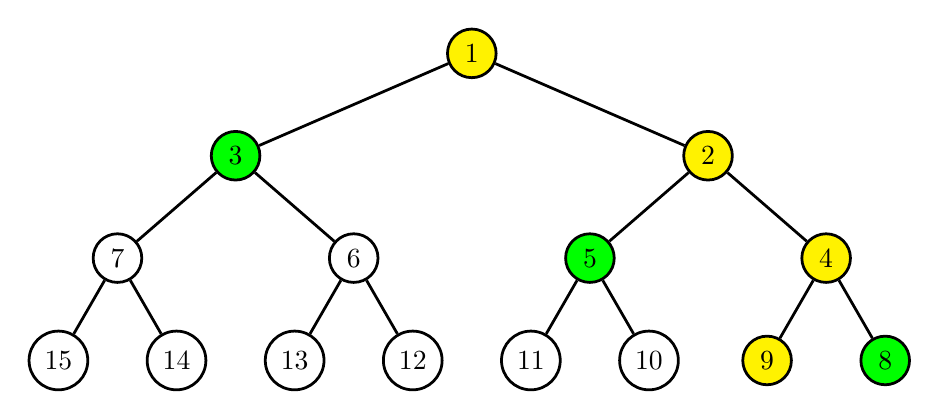
\begin{tikzpicture}[ grow'=down,
		 								line width = 1pt,
										vertex/.style={fill=none,draw,circle},
										level 1/.style={sibling distance=6cm, level distance=1.3cm},
										level 2/.style={sibling distance=3cm, level distance=1.3cm},
										level 3/.style={sibling distance=1.5cm, level distance=1.3cm}]
										
		\node [vertex, fill=yellow] {1}
			child {node[vertex, fill=yellow] {2}
				child {node[vertex, fill=yellow] {4}
					child {node[vertex, fill=green] {8}}
					child {node[vertex, fill=yellow] {9}}
				}
				child {node[vertex, fill=green] {5}
					child {node[vertex] {10}}
					child {node[vertex] {11}}
				}
			}
			child {node[vertex, fill=green] {3}
				child {node[vertex] {6}
					child {node[vertex] {12}}
					child {node[vertex] {13}}
				}
				child {node[vertex] {7}
					child {node[vertex] {14}}
					child {node[vertex] {15}}
				}
			};
		
		\end{tikzpicture}
		\caption{An example of 8 nodes}
	\end{figure}

	Now get back and see how the maximum is elected: each root of subtree is the maximum of the nodes which is the root's descendants. Observe Figure 1, the value of root of the whole tree(i.e. node of index 1) comes from the maximum of its children. Then we get a path(the node filling in yellow). Second maximum is the maximum of the other leaves. We can get the value by visiting the yellow path once and comparing the adjacent nodes(green nodes). The number of green nodes is the height of the tree, that is, $\log_2(n)$. We can conclude the second maximum by $\log_2(n)$ comparisons.

	In total, $n + \log_2(n) - 1$ comparisons achieved.
\end{problem}


\end{document}
